\chapter{Tecnica del dell'esame intraoperatorio}

\section{Introduzione}
Tagliare sezioni congelate con un criostato è un processo tecnico complesso che richiede abilità raffinate e una comprensione della istologia tissutale, della microanatomia e della patologia. L'obiettivo è preparare rapidamente vetrini di alta qualità per l'interpretazione microscopica, sia per diagnosi intraoperatoria in patologia chirurgica che per applicazioni di ricerca. Sviluppare abilità e sensibilità nell'uso del pennello consente di tagliare sezioni ripetute in movimento continuo senza esitazioni, in modo simile al suonare uno strumento musicale.

%%%%%%%%%%%%%%%%%%%%%%%
\section{Preparazione e configurazione del criostato}
%%%%%%%%%%%%%%%%%%%%%%%
Prima di iniziare il processo di sezionamento, è fondamentale assicurarsi che il criostato e i suoi componenti siano correttamente configurati e mantenuti.

\subsection{Inserire il supporto (tondello) e controllare il criostato}
Il blocco di tessuto deve essere \textbf{ben fissato} nel supporto del chuck. Tutti i pomelli, leve o viti di fissaggio per la lama, il portalama, il chuck, il supporto del chuck e il micrometro devono essere \textbf{ben serrati e privi di detriti} per evitare qualsiasi movimento che possa influenzare lo spessore delle sezioni. Anche un leggero movimento può compromettere sezioni sottili fino a 5 micron.

\subsection{Il pennello per sezioni congelate} 
Il pennello viene usato per afferrare il bordo della sezione mentre viene tagliata e guidarla sul piano del criostato.

\begin{itemize}
    \item \textbf{Selezione}: Sono consigliati pennelli a setole rigide, come quelli piatti da 3/16 o 1/4 di pollice (spesso reperibili nei negozi di articoli per artisti), piuttosto che pennelli flosci in pelo di cammello, grazie alla loro superficie di presa più ampia e funzionalità, soprattutto quando la sezione tende ad arricciarsi.
    \item \textbf{Preparazione}: Tagliare le setole del pennello a un angolo di circa 45 gradi, in modo che, tenuto inclinato, il pennello incontri il tessuto in modo piatto, come una scopa angolata. L'eccesso di manico dei pennelli lunghi da artista dovrebbe essere rimosso.
    \item \textbf{Pulizia}: Mantenere il pennello pulito riduce l'aderenza delle sezioni, in particolare nei tessuti grassi. Una rapida procedura di pulizia prevede sapone e acqua, asciugatura rapida con garza, immersione in alcol (ETOH) e xilene con asciugatura veloce, seguita dal raffreddamento del pennello sulla superficie fredda del criostato.
    \item \textbf{"Brush-brush"}: È possibile realizzare un "brush-brush" fissando un pezzo di garza o un piccolo pennello vicino alla mano sinistra all'interno del criostato, permettendo all'operatore di pulire rapidamente il pennello mantenendo il movimento continuo.
\end{itemize}

\subsection{La lama}
Si consiglia di utilizzare una nuova lama monouso per ogni campione del paziente, al fine di garantire la migliore qualità di sezione.
\begin{itemize}
    \item \textbf{Usura}: Tessuti duri, collagene o calcificati possono smussare rapidamente la lama, rendendo necessaria la sostituzione quando la qualità della sezione diminuisce.
    \item \textbf{Sicurezza}: Cambiare la lama per ogni caso è una misura di sicurezza importante, poiché riduce il rischio di trasmissione di malattie in caso di tagli accidentali.
    \item \textbf{Ascoltare la lama}: Una buona sezione non dovrebbe produrre suoni. Rumori stridenti o vibrazioni indicano problemi come un blocco troppo freddo, un angolo della lama errato, movimento o detriti nel supporto lama.
    \item \textbf{Angolo della lama}: L'angolo corretto della lama dovrebbe essere leggermente superiore all'angolo del bisello inferiore della lama, ma il meno possibile, per evitare la compressione del tessuto o la piegatura della sezione. Questo vale sia per i microtomi vibranti che per i criostati.
\end{itemize}

\subsection{Posizione del corpo e della mano}
\begin{itemize}
    \item \textbf{Posizione del corpo}: È consigliato sedersi comodamente su uno sgabello regolabile, a un'altezza che consenta alle braccia di poggiare comodamente sul piano del criostato, per massimizzare il controllo della mano che usa il pennello. Evitare di incurvarsi. 
    % \texFigure{Le Figure 4.4 e 4.5 illustrano la corretta postura e l'ergonomia per l'uso del criostato.}
    \item \textbf{Impugnatura del pennello}: Tenere il pennello come una penna con la mano sinistra, stabilizzando la mano appoggiando delicatamente il lato del mignolo sul piano del criostato. Ciò consente di usare le abilità motorie fini delle dita, come nella scrittura. Il pennello va tenuto a circa 45 gradi rispetto sia alla faccia del blocco che al piano (Figura \ref{fig:fse_pennello}). 
    % \texFigure{La Figura 4.6 mostra la corretta impugnatura del pennello.}
\end{itemize}

\begin{figure}[htbp]
    \centering
    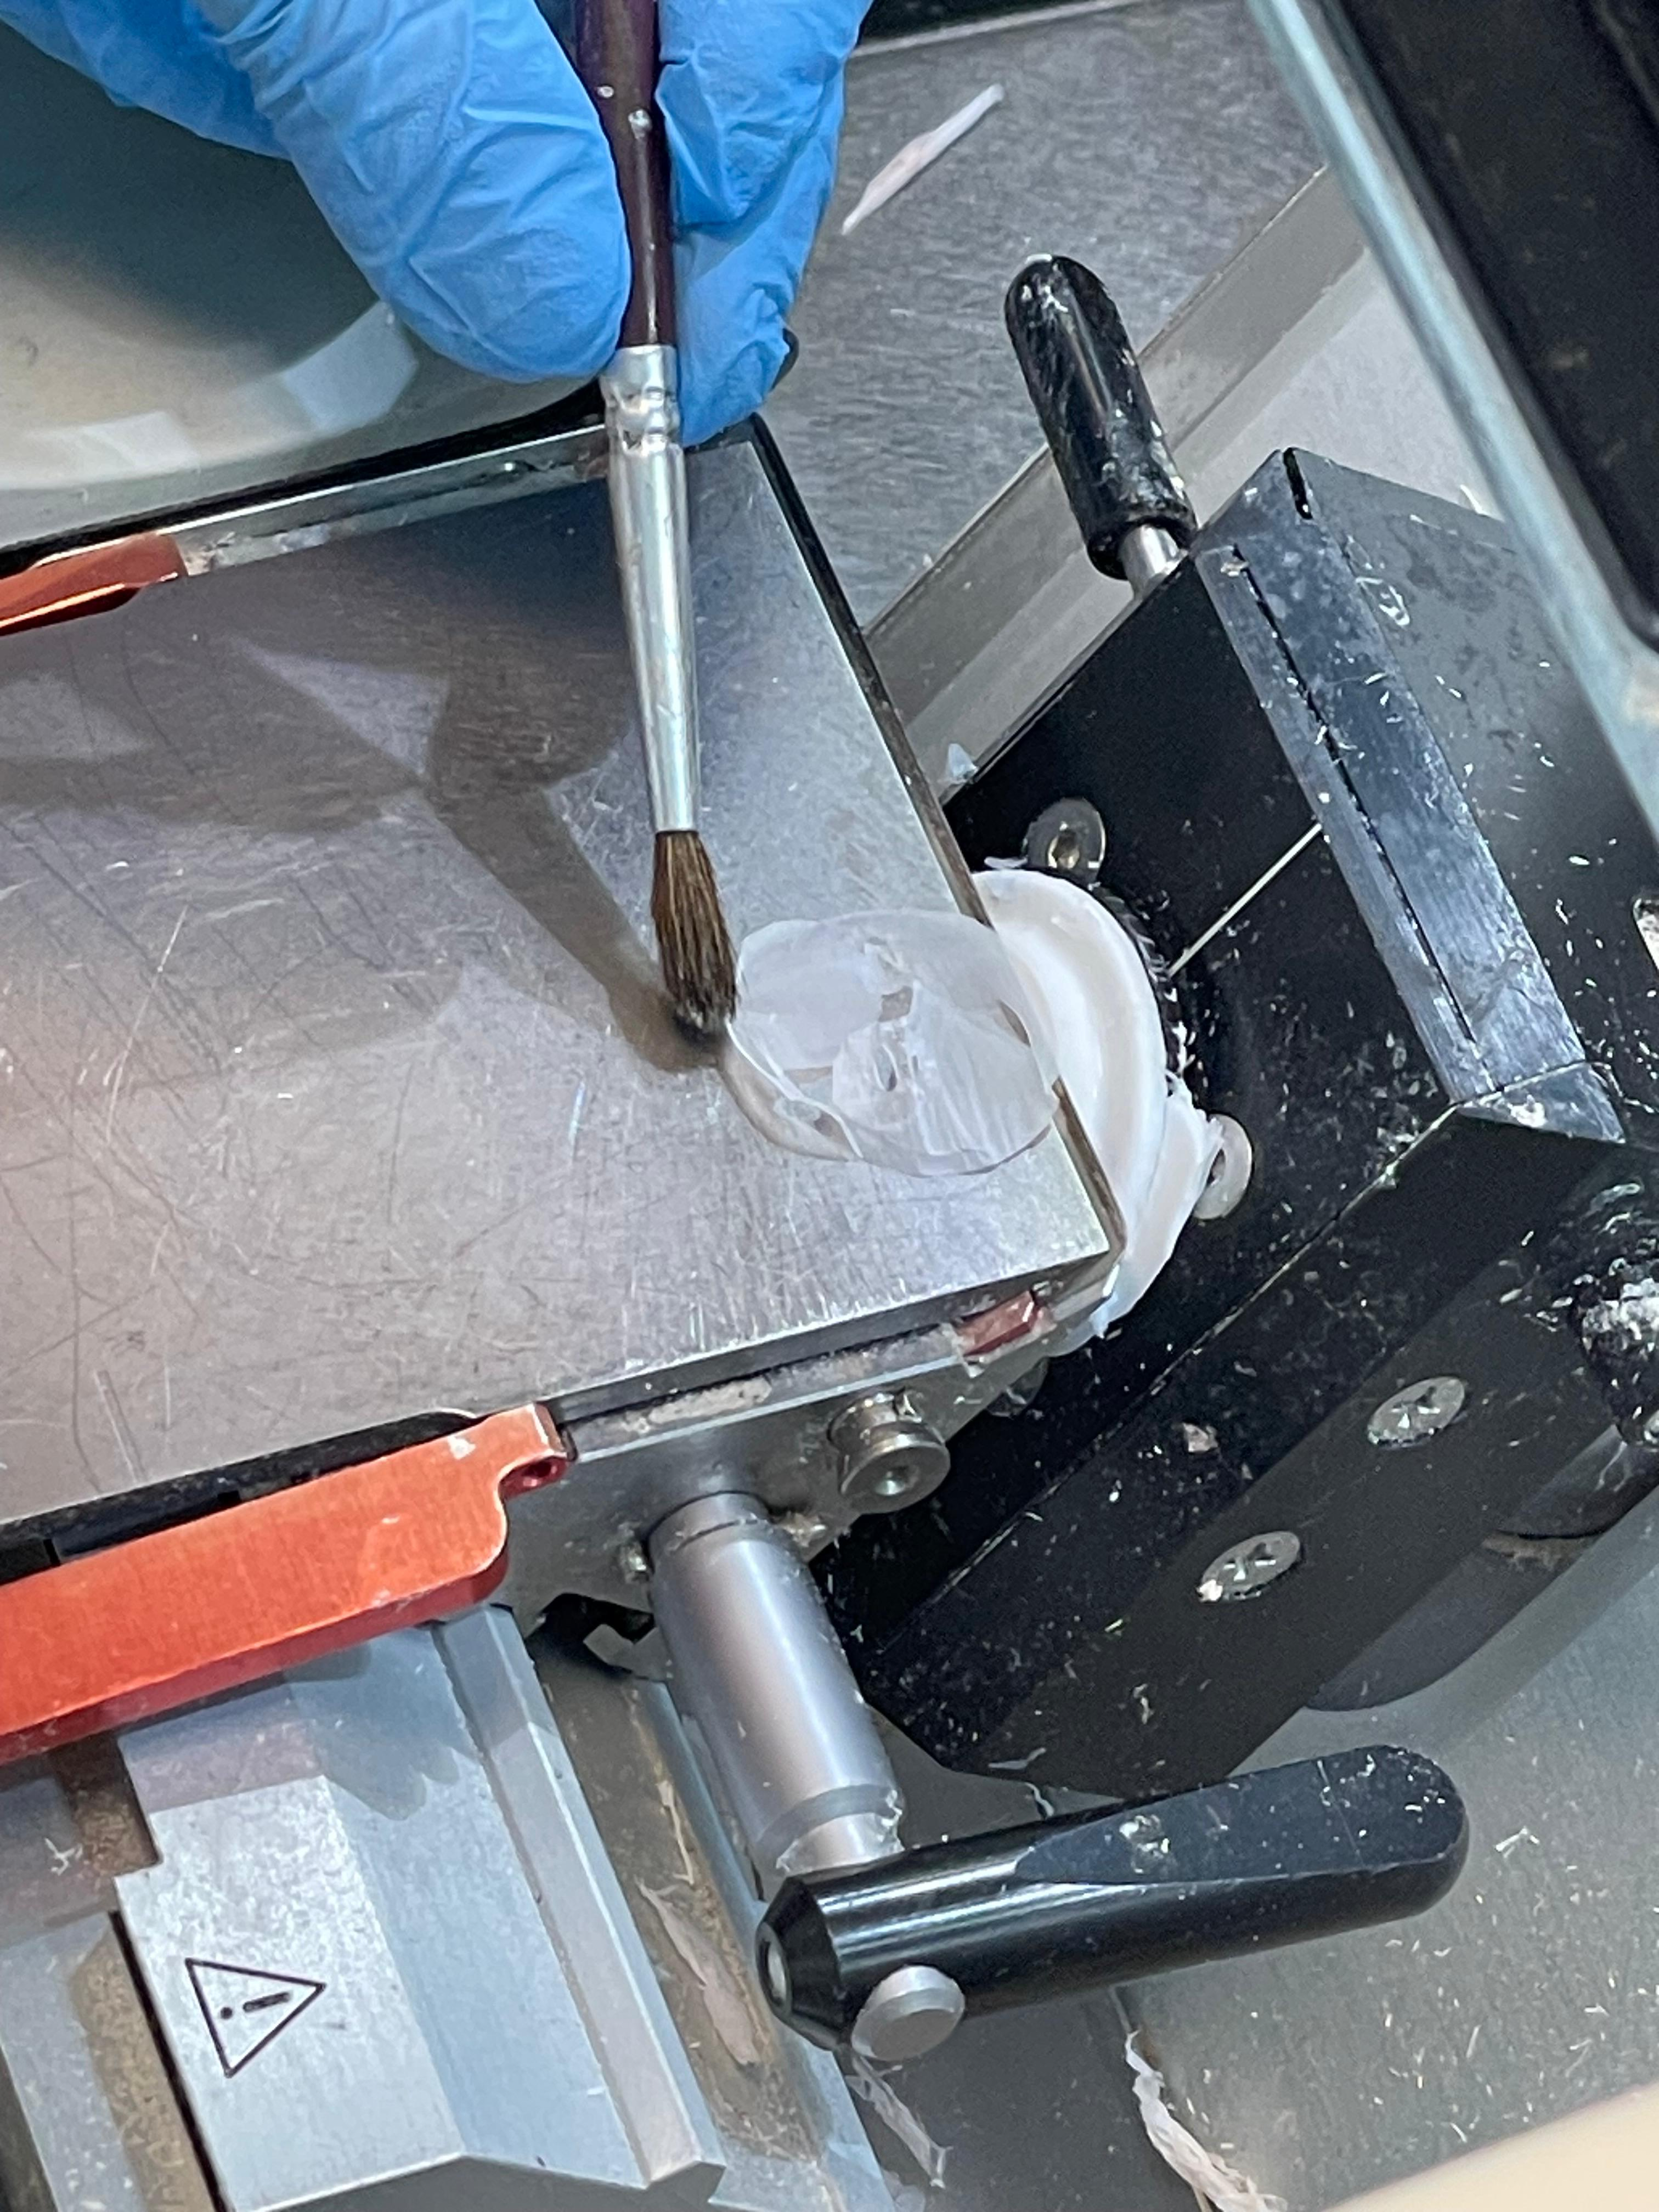
\includegraphics[width=0.75\textwidth]{fse_pennello}
    \caption{Uso del pennello. Il pennello viene tenuto a 45 gradi rispetto alla faccia del blocco e al piano del criostato, con la mano sinistra stabilizzata sul piano. Notare come la fetta venga stesa utilizzando il tondello come punto di ancoraggio.}
    \label{fig:fse_pennello}
\end{figure}

%%%%%%%%%%%%%%%%%%%%%%%
\section{Sgrossatura del blocco}
%%%%%%%%%%%%%%%%%%%%%%%
Sgrossare, o livellare, il blocco ha lo scopo di rimuovere rapidamente la superficie più esterna fino a raggiungere la profondità e i punti di riferimento desiderati.

\subsection{Avanzamento grossolano e fine}
Usare il meccanismo di avanzamento grossolano del criostato per rimuovere rapidamente gli strati iniziali. Quando i punti di riferimento diventano visibili, passare al controllo fine o girare manualmente la ruota del criostato per una sgrossatura precisa.

\subsection{Lettura del blocco}
Il tecnico al criostato deve imparare a riconoscere grossolanamente l'anatomia e i punti di riferimento sulla faccia del blocco e capire come il tessuto rifilato si relaziona all'area che il patologo esaminerà al microscopio. Questo comporta distinguere una ``faccia prematura'' (dove la struttura sembra presente ma è sfocata o non completamente esposta) da una ``faccia matura'' (dove tutti i punti di riferimento sono chiaramente visibili con linee nette e colori vividi) (Figura \ref{fig:faccia}). Il confronto tra la faccia del blocco e la sezione tagliata può aiutare. 
% \texFigure{La Figura 4.8 confronta una faccia prematura con una matura.}

 \begin{figure}[htpb]
      \centering
    \begin{subfigure}[b]{0.32\textwidth}
    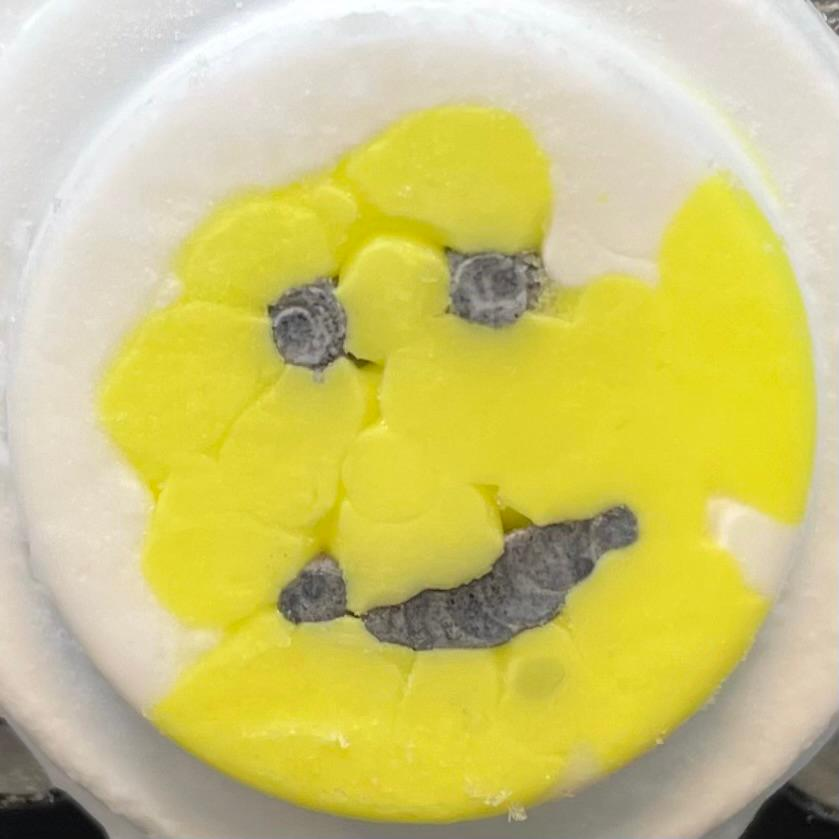
\includegraphics[width=\textwidth]{fse_coperto}
      \caption{Coperta}
    \end{subfigure}
    \begin{subfigure}[b]{0.32\textwidth}
    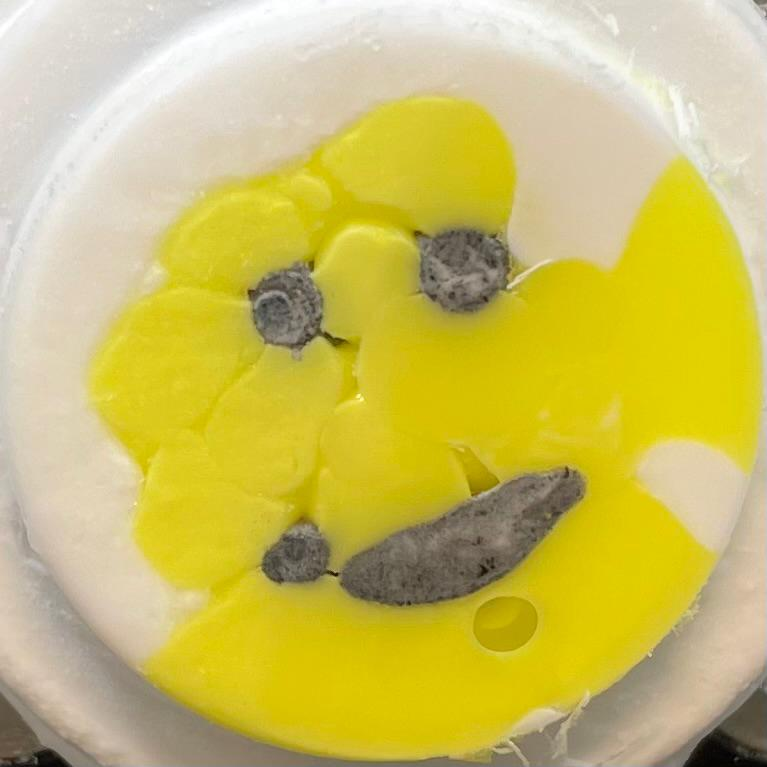
\includegraphics[width=\textwidth]{fse_medio}
      \caption{Prematura}
    \end{subfigure}
    \begin{subfigure}[b]{0.32\textwidth}
    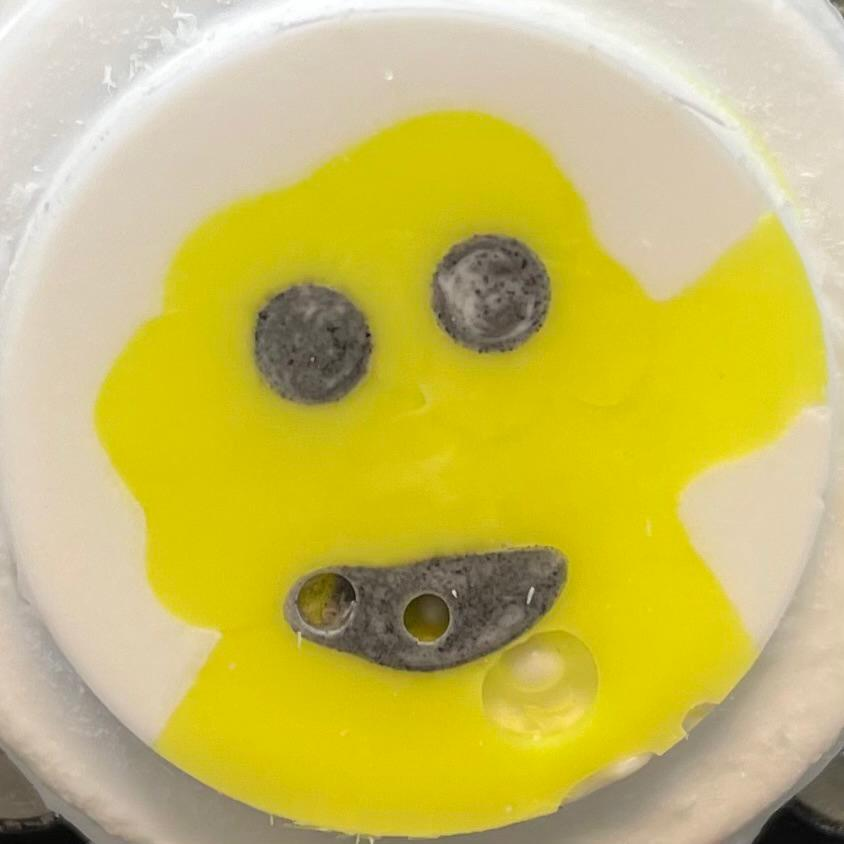
\includegraphics[width=\textwidth]{fse_scoperto}
      \caption{Scoperta}
    \end{subfigure}
\caption{Facce del blocco: a. L'intera superficie del blocco è coperta da mezzo di inclusione; b. Il tondello mostra una faccia prematura (soltanto il lato destro comincia a essere scoperto); c. L'intera superficie del tondello è scoperta, bisogna smettere di sgrossare e iniziare a tagliare le fette per l'istologia.}
\label{fig:faccia}
\end{figure}

\subsection{Orientamento Asse X-Y}
Per ridurre al minimo lo spreco di tessuto e ottenere completamente la faccia desiderata con poca sgrossatura, il tessuto deve essere incorporato in un piano piatto e il blocco correttamente orientato sull'asse X-Y (il piano della faccia del blocco deve essere parallelo al piano della lama).
Le regolazioni dell'orientamento del blocco devono essere fatte in incrementi molto piccoli. Un blocco ben orientato incontrerà per primo la lama al centro. Se invece inizia a tagliare da un bordo o un angolo, l'orientamento X-Y va corretto spostando indietro la parte tagliata e in avanti quella non ancora raggiunta. 
% \texFigure{Le Figure 4.9 e 4.10 illustrano una cattiva orientazione X-Y e l'effetto della rotazione del blocco.}

\subsection{Rotazione del blocco}
Molti criostati permettono la rotazione del blocco a 360 gradi, permettendo all'operatore di orientare il tessuto in modo ottimale rispetto alla lama. Questo è particolarmente utile se emergono elementi grassi o calcificazioni inattese, o se il tessuto si arriccia, permettendo di fare in modo che gli elementi problematici tocchino la lama per ultimi. Attenzione: ruotare il blocco può alterare il suo orientamento X-Y, rendendo necessaria una nuova regolazione.

\subsection{Rimozione e reinserimento del blocco}
Quando si rimuove il blocco, fare un piccolo segno alle ore 12 per poterlo riposizionare sul supporto nello stesso modo, evitando cambiamenti di orientamento e spreco di tessuto. Riportare sempre il blocco indietro prima di rifilare nuovamente per valutare eventuali variazioni di orientamento (alcuni todelli hanno un'incisura che serve a questo scopo).

\subsection{Sgrossare i piccoli campioni}
Per biopsie minute o core biopsies sottili (meno di un millimetro di diametro), è essenziale incorporare il tessuto nel piano più piatto possibile e iniziare con un blocco ben orientato. Se il tessuto è visibile ma non coperto da mezzo di inclusione, iniziare con uno strato di copertura. Rifilare delicatamente, osservando il tessuto mentre viene scoperto, e tagliare sezione per sezione per preservare materiale per sezioni in paraffina. 
% \texFigure{La Figura 4.11 mostra il processo di taglio di campioni minuti.}

%%%%%%%%%%%%%%%%%%%%%%%
\section{Taglio delle sezioni finali}
%%%%%%%%%%%%%%%%%%%%%%%
L'obiettivo è girare la ruota del criostato in modo continuo e uniforme, senza esitazioni, imitando un criostato automatizzato. Il pennello guida la sezione appena tagliata verso il piano del criostato.

\subsection{Taglio con pennello - SSTT}
Il taglio con il pennello richiede quattro movimenti principali, che possono essere ricordati con l'acronimo SSTT: Seguire, Solleva, Tieni e Tira. Questi movimenti devono essere eseguiti in modo fluido e continuo per ottenere sezioni di alta qualità.

\begin{enumerate}
\item \textbf{Seguire}: Dalla posizione iniziale (al centro, ultimi due millimetri inferiori del blocco), il pennello si muove verso il basso, seguendo il blocco mentre scende verso la lama.
\item \textbf{Solleva}: Quando il pennello incontra la lama, si solleva delicatamente il pennello tenendo il bordo della sezione appena formata.
\item \textbf{Tieni}: Quando la sezione si arriccia, il pennello in movimento si posiziona sopra il ricciolo, trattenendolo. Poi il pennello cambia direzione in un movimento orizzontale verso l'operatore, seguendo una forma a “gomito” (parte sinistra della figura \ref{fig:fse_taglio}).
\item \textbf{Tira}: Continuare il movimento orizzontale, trascinando delicatamente la sezione sul piano, senza premere il tessuto contro il piano, per evitare aderenze o sbavature, soprattutto nei tessuti adiposi (parte destra della figura \ref{fig:fse_taglio}).
% \texFigure{La Figura 4.12 illustra questi quattro movimenti e il percorso ellittico continuo del pennello.}
\end{enumerate}

\begin{figure}[htbp]
    \centering
    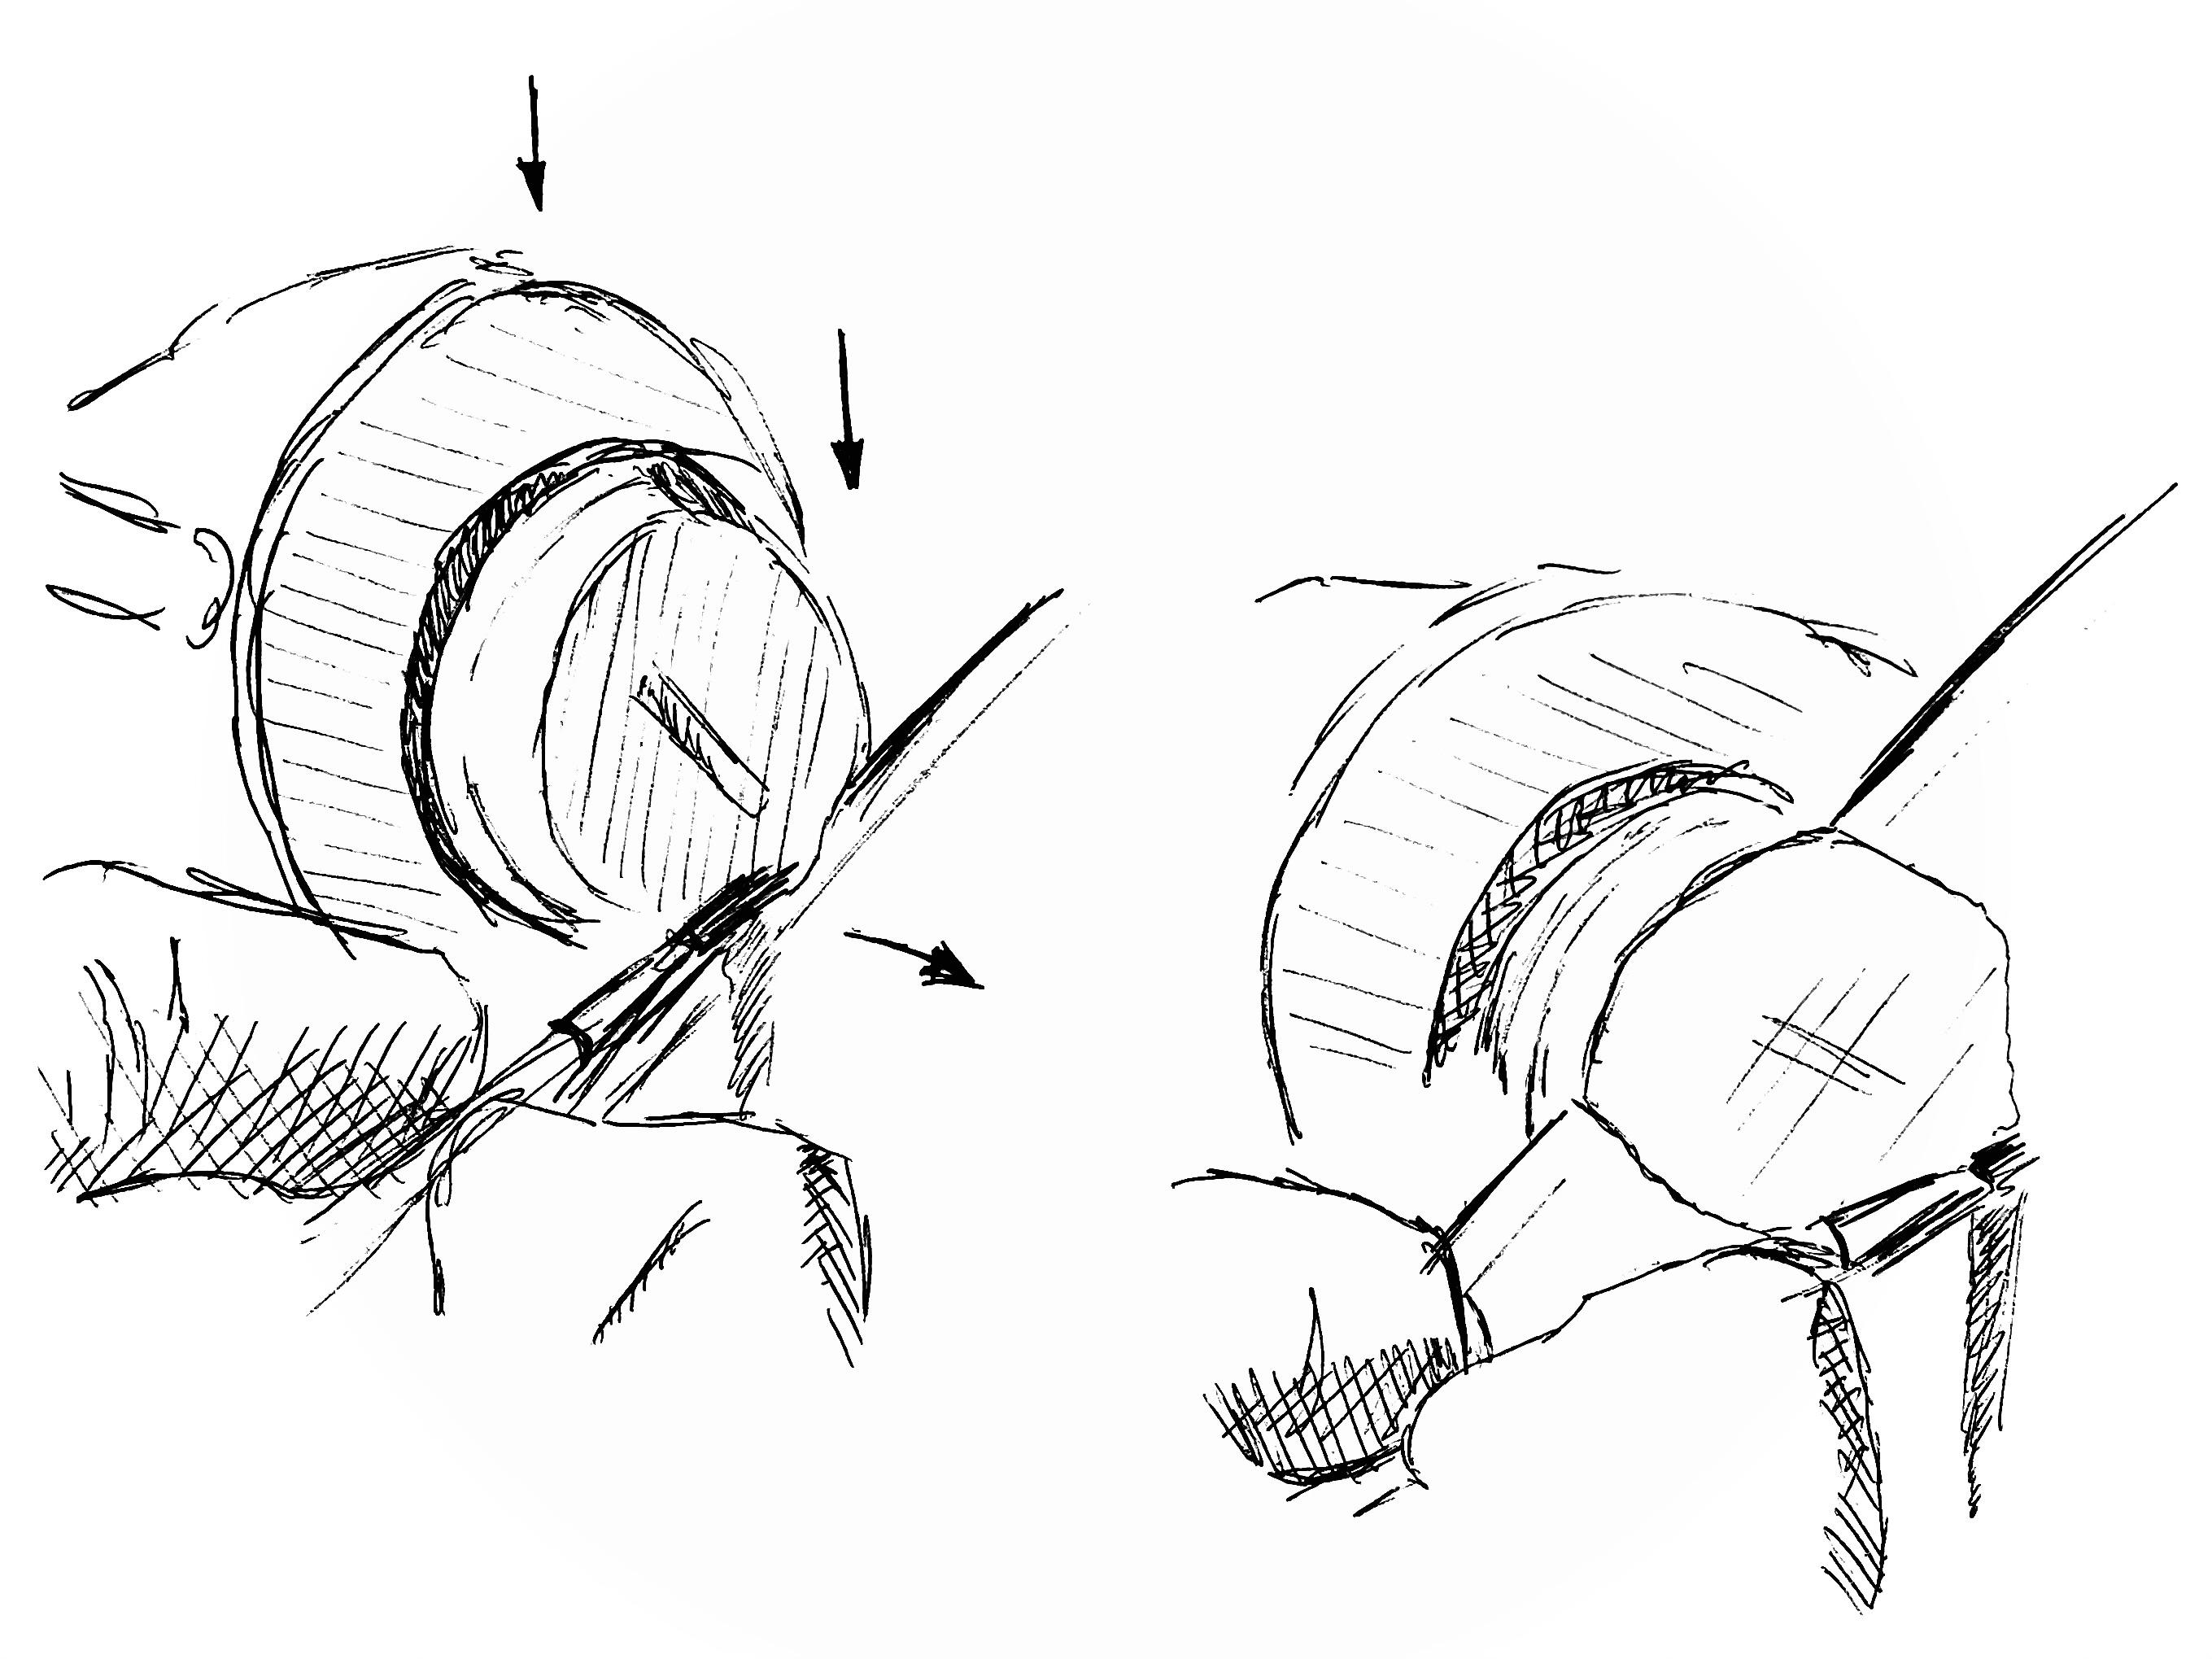
\includegraphics[width=0.75\textwidth]{fse_taglio}
    \caption{Taglio con il pennello. La parte sinistra della figura mostra il momento in cui la fetta comincia ad arricciarsi. Il blocco del tondello si muove verso il basso e la sezione viente tenuta dal pennello. la parte destra mostra l'uso del pennello per stendere la sezione sul piano del criostato.}
    \label{fig:fse_taglio}
\end{figure}

\subsection{Uso del ``manico''} 
Preparare i blocchi con un bordo di mezzo di inclusione (``manico'') attorno al tessuto è vantaggioso. Questo bordo fornisce un margine di sicurezza per afferrare la sezione senza toccare direttamente il tessuto, stabilizza tessuti più fragili (es. necrotici o grassi) e offre uno ``slancio iniziale'' per sezioni difficili.

%%%%%%%%%%%%%%%%%%%%%%%
\section{Recupero della sezione}
%%%%%%%%%%%%%%%%%%%%%%%
Recuperare la sezione consiste nel trasferire la sezione congelata tagliata su un vetrino per microscopio. Questo va fatto tenendo conto della delicatezza del tessuto e della cinetica del processo, per evitare piegature, stiramenti o lacerazioni.

\subsection{Recupero dal piano}
Tenere il vetrino appena sopra la sezione e inclinarlo verso il basso per toccare una parte del tessuto. L'attrazione elettrostatica farà aderire la sezione e scioglierla rapidamente sul vetrino caldo. Si può usare la punta del dito per stabilizzare il bordo anteriore del vetrino mentre lo si abbassa. Se è difficile recuperare la sezione, lasciar cadere il vetrino da circa mezzo centimetro sopra il tessuto. Pennelli puliti aiutano a prevenire l'adesione. Le sezioni tagliate alla temperatura ideale restano piatte e sono più facili da recuperare e posizionare.
% \texFigure{La Figura 4.13 mostra il recupero delle sezioni dal piano del criostato.}

\subsection{Recupero dal blocco} 
In caso di difficoltà nel recupero dal piano (es. arricciamento, aderenza o elettricità statica), tagliare il tessuto lasciando 1–2 mm prima del distacco completo. Girare la ruota del criostato all'indietro per riportare la sezione ancora attaccata sopra la faccia del blocco. Il bordo fisso della sezione può quindi essere delicatamente tirato verso il basso con il pennello, mentre il vetrino viene posizionato sopra il blocco per raccogliere la sezione.
% \texFigure{La Figura 4.14 illustra il recupero delle sezioni dalla faccia del blocco.}

%%%%%%%%%%%%%%%%%%%%%%%
\section{Variabili che influenzano le proprietà di taglio dei tessuti}
%%%%%%%%%%%%%%%%%%%%%%%
La qualità delle sezioni congelate è fortemente influenzata da vari fattori, principalmente dalla temperatura del blocco. Riconoscere gli artefatti quando compaiono consente correzioni tempestive.

%%%
\subsection{Temperatura del blocco}
\subsubsection{Blocco troppo caldo} 
Se il mezzo di inclusione ha un tono grigiastro, il tessuto si accartoccia o viene “strappato via” (completamente estratto dal blocco) perché non è abbastanza solido o non si è ancora indurito rispetto al mezzo.

\begin{itemize}
\item \textbf{Stadio di accartocciamento}: Raffreddandosi, le sezioni iniziano a formarsi ma si accartocciano leggermente, segnalando che il tessuto non è ancora abbastanza rigido da mantenere la forma.
\item \textbf{Temperatura ideale}: Quando il tessuto inizia a produrre sezioni complete e pulite con facilità (tipicamente tra -16 e -20°C per la maggior parte dei tessuti), ha raggiunto la temperatura ideale. A questa temperatura, le sezioni restano piatte, si arricciano poco e non si spezzano, consentendo il taglio a nastro.
\end{itemize}

% \texFigure{Le Figure 5.1 e 5.2 mostrano l'effetto della temperatura sulla qualità delle sezioni e lo stadio di accartocciamento.}
\subsubsection{Blocco troppo freddo}
Sotto i -25°C aumentano arricciamento e fratture, ostacolando l'interpretazione. Blocchi eccessivamente raffreddati possono anche causare sezioni irregolari o ``vibrazioni'' (chatter).

\subsubsection{Regolare la temperatura}
\begin{itemize}
\item \textbf{Riscaldare}: Per blocchi troppo freddi, premere delicatamente il pollice guantato o il palmo sulla faccia del tessuto per alcuni secondi. Si può anche usare un estrattore di calore rivestito con nastro adesivo. Agire rapidamente: il riscaldamento è temporaneo.
\item \textbf{Raffreddare}: Per blocchi troppo caldi o che si accartocciano, applicare un blocco di raffreddamento sopra il blocco o un estrattore di calore per alcuni secondi. Si possono usare spray congelanti, soprattutto per tessuti grassi, con cautela per evitare sovraraffreddamento e aerosolizzazione.
Vedi la sezione \ref{sec:artefatti} per ulteriori dettagli sugli artefatti legati alla temperatura.
\end{itemize}

%%%
\subsection{Conoscere i tessuti}
\subsubsection{Tessuti molli non grassi} 
Si tagliano facilmente con una lama affilata e buona tecnica, anche in pezzi grandi.
\subsubsection{Tessuti acquosi} 
Alcuni tessuti (es. cervello, tessuti edematosi) tendono a frantumarsi; sezionare alla temperatura più calda possibile. La frantumazione aumenta con lo spessore della sezione.
\subsubsection{Tessuti collagenosi duri}
Altri (es. cuoio capelluto, cervice) si tagliano bene in piccoli pezzi. In pezzi grandi possono causare chatter o sezioni irregolari. Scaldare il blocco fino allo stadio di accartocciamento, poi raffreddare delicatamente alla temperatura ideale. Orientare l'asse lungo diagonalmente o perpendicolare alla lama.
\subsubsection{Tessuti ossei duri} 
Danneggiano rapidamente le lame monouso. Per osso trabecolare, sgrossare, cambiare lama e tagliare con pochi giri. L'osso corticale solitamente non si taglia con lame monouso; si può rimuovere ``scavando'' e poi stuccando il difetto.
\subsubsection{Tessuti necrotici o liquefatti} 
Possono lasciare buchi e staccarsi durante la colorazione per perdita di integrità strutturale. Includere tessuto vitale se possibile. Un manico di mezzo e il movimento continuo aiutano. Minimizzare l'agitazione durante la colorazione.
\subsubsection{Tessuti adiposi} 
Il ``nemico giurato'' del criotomista. Il grasso si spalma e impedisce il taglio perché non congela sufficientemente alle temperature normali e aderisce male al mezzo.
\begin{enumerate}
\item \textbf{Rimuovere il grasso non necessario}: Eliminare accuratamente il grasso (tipicamente dai linfonodi) migliora la qualità della sezione.
\item \textbf{Lama affilata e blocco molto freddo}: Essenziali per sezionare tessuti grassi. Usare spray congelanti, teste criogeniche, azoto liquido, ecc.
\item \textbf{Pulire piano e lama}: Rimuovere qualsiasi residuo o tessuto spalmato.
\item \textbf{Sezioni spesse di grasso}: Sezioni più spesse (es. 10-50 $\mu m$) possono risultare trasparenti e interpretabili, mostrando strutture in 3D. Aumentare i tempi di colorazione e ridurre l'agitazione.
\item \textbf{Tecnica “scavo del grasso”}: Il grasso morbido può essere raschiato via con una pinza e il difetto riparato con stucco.
\item \textbf{Applicare azoto liquido}: Indurisce direttamente gli elementi grassi.
\end{enumerate}


%%%
\subsection{Arricciamento inverso}
Si verifica quando il tessuto si separa dal mezzo di inclusione, spesso per presenza di grasso, epidermide o tessuto necrotico. Il diverso comportamento tra tessuto e mezzo causa il problema. In questo caso si può scaldare il blocco alla temperatura ottimale. Se causato da grasso, usare la tecnica dello scavo e stuccare. Per l'epidermide, incidere con un bisturi in punti specifici (es. ore 3, 6, 9) e stuccare. Inoltre ruotare il tondello in modo tale da orientare la superficie epidermica perpendicolare alla lama aiuta.

%%%
\subsection{Spessore della sezione}
Ideale intorno a 5 $\mu m$ per la diagnosi, anche se 6 $\mu m$ è spesso preferito per una colorazione più intensa. Sezioni più sottili (es. 3 $\mu m$) sono più flessibili; quelle più spesse (es. 10 $\mu m$) più rigide. La conferma visiva è importante poiché il criostato può essere impreciso. Il movimento continuo aiuta a mantenere lo spessore costante.
\subsubsection{Sezioni spesse e sottili / Striature e vibrazioni}:
\begin{itemize}
\item \textbf{Sezioni spesse e sottili alternate}: Possono essere causate da stress sulla lama o angolo errato. Una lama arcuata può tagliare i bordi lasciando il centro intatto.
\item \textbf{Striature sottili}: Perpendicolari alla lama, indicano incisioni sulla lama, spesso causate da tessuti calcificati, punti di sutura, graffette o urti accidentali.
\item \textbf{Striature larghe / lacerazioni}: Dovute all'adesione del tessuto sotto la lama, frequenti nei tessuti grassi. La lama va pulita o sostituita.
\item \textbf{Chatter (linee ondulate)}: Linee ondulate regolari indicano movimento nel sistema. Tutti i componenti devono essere saldi e privi di detriti. Può anche essere causato da tessuto troppo duro o freddo per essere tagliato senza stress.
\end{itemize}

%%%%%%%%%%%%%%%%%%%%%%%%%%
\section{Artefatti e contromisure}
\label{sec:artefatti}
%%%%%%%%%%%%%%%%%%%%%%%%%%%
Come tecnico di laboratorio che esegue sezioni al congelatore, la comprensione e la mitigazione degli artefatti sono cruciali per produrre vetrini di alta qualità e garantire un'interpretazione microscopica accurata.  La vostra capacità di riconoscere questi problemi non appena si presentano e di applicare misure correttive ridurrà significativamente gli errori e farà risparmiare tempo prezioso. 

%%%%
\subsection{Artefatti legati alla temperatura}
La temperatura del blocchetto di tessuto è probabilmente una delle variabili più critiche che influenzano la qualità delle sezioni al congelatore. 

\subsubsection{Stadio di accartocciamento}
Quando un blocchetto congelato è \textbf{troppo caldo}, tipicamente indicato dal mezzo di inclusione che ha ancora una tonalità leggermente grigiastra, il tessuto si accartoccerà completamente durante il taglio.  Ciò si verifica perché il tessuto non è abbastanza solido da mantenere una forma piatta, simile a un foglio di carta.  Man mano che il blocchetto si raffredda, le sezioni possono iniziare a formarsi ma si accartocceranno ancora leggermente poiché il tessuto non è abbastanza rigido da mantenere la sua vera forma e l'attrito del coltello lo fa ammassare. 

\subsubsection{Frantumazione}
Al contrario, se il blocchetto di tessuto è \textbf{troppo freddo}, le sezioni diventeranno dure e rigide, portando a una tendenza a \textbf{frantumarsi} o rompersi mentre vengono tagliate.  Questo perché la lama, agendo come un cuneo, costringe il tessuto a piegarsi;  se il tessuto è troppo duro per flettersi, si romperà.  La frantumazione aumenta con la diminuzione delle temperature, lo spessore maggiore della sezione e un più alto contenuto di acqua nel tessuto. Ciò può ostacolare gravemente l'interpretazione. 
%figura che spiega gli artefatti di frantumazione a diverse temperature, simile alla Figura 5.1 nella fonte

\subsubsection{Distacco di frammenti}
Un artefatto particolarmente frustrante si verifica quando il tessuto viene \textbf{``staccato a pezzi''} dal blocchetto.  Questo accade quando il tessuto o il mezzo di inclusione non è completamente congelato, il che significa che il mezzo non ha aderito saldamente al tessuto.  Quando la lama tenta di tagliare, gli elementi fibrosi nel tessuto non congelato resistono al taglio e causano il distacco del tessuto dal blocchetto.  Questo è spesso visibile come una dominante grigiastra nel blocco di inclusione. 

\subsubsection{Contromisure}
\begin{itemize}
    \item   \textbf{Temperatura ideale}: L'obiettivo è tagliare la maggior parte dei tessuti (esclusi i tessuti adiposi) a una temperatura ideale, tipicamente intorno a $-17^\circ \text{C}$ a $-20^\circ \text{C}$.  A questa temperatura, le sezioni di tessuto scorreranno in modo pulito sulla lama, con minimo arricciamento o frantumazione, e si adageranno piatte sul piatto del criostato, consentendo un facile recupero e persino la formazione di nastri.  Anche i tessuti acquosi come il cervello e i tessuti duri si sezionano meglio in questo intervallo. 
    \item   \textbf{Riscaldare un blocchetto troppo freddo}: Se un blocchetto è troppo freddo e si frantuma, è possibile riscaldarne la superficie premendo delicatamente il pollice guantato o il palmo della mano sul tessuto per alcuni secondi.  Prestare attenzione alla vicinanza della lama e assicurarsi che il volantino del microtomo sia bloccato per prevenire infortuni.  Un'alternativa più sicura è un estrattore di calore coperto con nastro adesivo a temperatura ambiente.  Dopo il riscaldamento, la prima sezione potrebbe essere più spessa, quindi tagliare rapidamente alcune sezioni fino a ottenere lo spessore e la qualità appropriati. 
    \item   \textbf{Raffreddare un blocchetto caldo}: Se un blocchetto è troppo caldo e si accartoccia, raffreddarlo applicando un blocco di congelamento sopra il chuck o un estrattore di calore sulla superficie del blocchetto per alcuni secondi.  Si possono anche usare spray congelanti, ma con giudizio, poiché possono raffreddare eccessivamente il blocchetto. 
    \item   \textbf{Movimento continuo}: Tagliare con un movimento continuo e uniforme aiuta a stabilire un equilibrio di temperatura e consistenza, portando a spessore e qualità più uniformi. 
\end{itemize}

\subsection{Difficoltà di taglio specifiche per tessuto}

Diversi tipi di tessuto presentano sfide uniche a causa delle diverse composizioni di grasso, acqua e collagene, nonché della loro durezza intrinseca. 

\subsubsection{Tessuti adiposi}
I tessuti adiposi sono la "nemesi" del criotomista.
\begin{itemize}
    \item   \textbf{Spalmatura}: Il grasso non congela bene e deve essere raffreddato a temperature molto basse per indurirsi abbastanza per il sezionamento.  Se non è abbastanza freddo, il grasso si spalmerà e impedirà il taglio di qualsiasi tessuto sul suo percorso. 
    \item   \textbf{Arricciamento e scarsa aderenza}: Il grasso non aderisce bene al mezzo di inclusione.  Se un tessuto più gestibile (come un linfonodo) è circondato da grasso, il grasso può impedire l'adesione, causando l'arricciamento del tessuto lontano dal mezzo, lasciando dei buchi. 
    \item   \textbf{Contromisure}:
    \begin{itemize}
        \item   \textbf{Dissezione del grasso in eccesso}: Rimuovere meticolosamente il grasso non essenziale, specialmente intorno ai linfonodi, per migliorare la qualità della sezione. 
        \item   \textbf{Lama affilata e blocchetto freddo}: Usare una lama nuova e affilata.  Raffreddare il blocchetto a temperature molto basse usando spray congelante, un estrattore di calore a bassissima temperatura o la testa di congelamento del criostato.  L'azoto liquido può essere applicato direttamente sulle aree adipose con un pennello. 
        \item   \textbf{Orientare il grasso per ultimo}: Quando possibile, orientare il tessuto in modo che il grasso colpisca la lama per ultimo o da solo, e assicurarsi sempre che ci sia una "maniglia" di mezzo di inclusione che circonda il tessuto.  Questa maniglia fornisce supporto e tiene insieme la sezione, anche se il grasso si spalma. 
        \item   \textbf{Sezioni spesse di grasso}: Per alcune interpretazioni (ad es. margini mammari nella chirurgia di Mohs), può essere utile prelevare sezioni più spesse di grasso (ad es. $50\,\mu\text{m}$).  Queste possono fornire una visione tridimensionale in cui il grasso è trasparente, consentendo la visualizzazione di strutture come capillari e cellule tumorali.  Aumentare i tempi di colorazione e utilizzare un'agitazione minima per le sezioni più spesse. 
        \item   \textbf{La manovra di sgombero del grasso}: Se il grasso impedisce il taglio, è possibile rimuoverlo dal blocchetto usando una pinza o un altro strumento, quindi riparare il difetto "intonacando" con mezzo di inclusione. 
    \end{itemize}
\end{itemize}
%figura che mostra l'inclusione di tessuto adiposo con una maniglia, simile alla Figura 5.3 nella fonte
%figura che illustra la manovra di sgombero del grasso, simile alla Figura 5.6 nella fonte

\subsubsection{Tessuti collagene duri}
Tessuti come il cuoio capelluto e la cervice sono duri e possono stressare la lama, specialmente a basse temperature o con lame più sottili.  Questo può portare a sezioni spesse e sottili o a vibrazioni (chatter).
\begin{itemize}
    \item   \textbf{Contromisure}: Tagliare pezzi più piccoli.  Per pezzi grandi, riscaldare il blocchetto fino allo stadio di accartocciamento, quindi raffreddare di nuovo delicatamente fino a quando le sezioni si formano.  Posizionare l'asse lungo del tessuto in diagonale o perpendicolarmente alla lama per minimizzare il diametro effettivo e ridurre lo stress. 
\end{itemize}

\subsubsection{Tessuti acquosi}
I tessuti con un alto contenuto di acqua, come il cervello o i tessuti edematosi, hanno una maggiore tendenza a frantumarsi a causa della formazione di cristalli di ghiaccio. 
\begin{itemize}
    \item   \textbf{Contromisure} Sezionare alla temperatura più calda possibile.  Iniziare leggermente caldi e raffreddare con un estrattore di calore se necessario.  La frantumazione aumenta anche con lo spessore della sezione, quindi considerare di tagliare più sottile se problematico. 
\end{itemize}
%figura che illustra le "bolle" nello stroma edematoso, simile alla Figura 7.5 nella fonte
%figura che illustra gli artefatti da compressione, simile alla Figura 7.6 nella fonte

\subsubsection{Tessuti necrotici e liquefattivi}
Questi tessuti hanno perso l'integrità strutturale e possono lasciare buchi al sezionamento o staccarsi durante la colorazione. 
\begin{itemize}
    \item   \textbf{Contromisure}: Campionare macroscopicamente per includere tessuto vitale per il supporto strutturale.  Una maniglia di mezzo di inclusione aiuterà a sostenere la sezione. Usare una lama affilata e un movimento continuo.  Ridurre al minimo l'agitazione durante la colorazione.
\end{itemize}

\subsubsection{Tessuti duri e ossei}
I tessuti contenenti osso trabecolare possono essere sezionati, ma \textbf{danneggeranno rapidamente le lame monouso}.  L'osso corticale è generalmente troppo duro per le lame monouso.
\begin{itemize}
    \item   \textbf{Contromisure}: Per l'osso trabecolare, rifilare il blocchetto, quindi passare a una nuova sezione della lama prima di prelevare la sezione finale.  Usare il minor numero di giri possibile e prevedere cambi multipli della lama.  Per l'osso corticale, rimuovere l'osso e riparare il blocchetto "intonacando". 
\end{itemize}

\subsection{Artefatti meccanici e tecnici}

Anche i problemi legati alla meccanica del criostato o alla tecnica dell'operatore possono introdurre artefatti. 

\subsubsection{Sezioni spesse e sottili / Vibrazioni (Chatter)}
Questo si manifesta come sezioni alternate più spesse e più sottili dell'impostazione desiderata. 
\begin{itemize}
    \item   \textbf{Cause}:
    \begin{itemize}
        \item   \textbf{Sovraccarico della lama}: Troppa resistenza del tessuto può stressare la lama. 
        \item   \textbf{Angolo della lama improprio}: Un angolo della lama errato può causare compressione. 
        \item   \textbf{Componenti allentati}: Qualsiasi allentamento nel portalama, nel chuck, nel portachuck o nei meccanismi del microtomo causerà movimento e porterà a spessore di sezione incoerente o "vibrazioni". 
        \item   \textbf{Fluttuazione di temperatura}: Quando il blocchetto riposa per più di pochi secondi, i cambiamenti di temperatura superficiale possono causare espansione, portando a una prima sezione più spessa seguita da altre più sottili. 
    \end{itemize}
    \item   \textbf{Contromisure}:
    \begin{itemize}
        \item   \textbf{Garantire la tenuta}:Controllare regolarmente che tutte le manopole, le leve e le viti di bloccaggio siano strette e prive di detriti. 
        \item   \textbf{Ottimizzare l'angolo della lama}: L'angolo corretto della lama dovrebbe essere leggermente al di sopra dell'angolo dello smusso inferiore della lama, ma il più piccolo possibile, per evitare la compressione o l'eccessiva piegatura del tessuto. 
        \item   \textbf{Movimento continuo}: Mantenere un movimento fluido e continuo durante il taglio per garantire uno spessore uniforme. 
    \end{itemize}
\end{itemize}

\subsubsection{Strie}
\begin{itemize}
    \item   \textbf{Strie sottili}: Sono linee perpendicolari alla lama, che indicano tipicamente intaccature sulla lama.  Ciò può essere causato da calcificazioni, suture o graffette nel tessuto, o toccando accidentalmente il bordo della lama su una superficie dura. 
    \item   \textbf{Consiglio professionale}: Cambiare con una lama nuova e affilata. 
    \item   \textbf{Strie larghe / Lacerazione}: Si verifica quando il tessuto (spesso tessuto adiposo) aderisce alla parte inferiore della lama. 
    \item   \textbf{Consiglio professionale}: Rimuovere con cura la lama e pulirla o sostituirla.  Invertire sempre il blocchetto prima di pulire o cambiare la lama. 
\end{itemize}
%figura che mostra strie sottili dovute a lama intaccata, simile alla Figura 5.9 nella fonte
%figura che mostra strie larghe e lacerazioni dovute all'adesione del tessuto alla lama, simile alla Figura 5.10 nella fonte

\subsubsection{Arricciamento (non legato al grasso)}
Oltre ai tessuti adiposi, anche altre parti di tessuto possono separarsi dal mezzo di inclusione e arricciarsi.  Questo è chiamato \textbf{"arricciamento"}. Ad esempio, l'epidermide della pelle tende a separarsi a causa dello strato corneo desquamante. 
\begin{itemize}
    \item   \textbf{Contromisure}:
    \begin{itemize}
        \item   \textbf{Riscaldare il blocchetto}: Riscaldare il blocchetto alla temperatura ottimale può minimizzare l'arricciamento sia del tessuto che del mezzo. 
        \item   \textbf{Ruotare il blocchetto}: Se solo una parte si sta arricciando, ruotare il blocchetto in modo che il punto di separazione sia lontano dal coltello (l'ultimo a colpire il coltello). 
        \item   \textbf{Intaccare e intonacare}: Per la pelle o il tessuto coperto di grasso incline all'arricciamento, intaccare la superficie epidermica o il grasso nella faccia del blocchetto in diversi punti (ad es. alle posizioni 3, 6 e 9) e quindi intonacare i difetti con mezzo di inclusione.  Ciò espone il tessuto sottostante che aderisce meglio al mezzo. 
        \item   \textbf{Orientamento per l'inclusione}: Quando si include la pelle, orientare l'epidermide perpendicolarmente alla lama e, se possibile, orientare le punte lontano dalla lama per minimizzare il ribaltamento. 
    \end{itemize}
\end{itemize}
%figura che illustra l'arricciamento e come il riscaldamento aiuta, simile alla Figura 5.7 nella fonte

\subsubsection{Scarsa aderenza / Caduta del tessuto dal vetrino}
Le sezioni occasionalmente cadono dal vetrino durante il processo di colorazione. 
\begin{itemize}
    \item   \textbf{Cause}:
    \begin{itemize}
        \item   \textbf{Natura del tessuto}: Tessuti molto secchi, sclerotici o necrotici/liquefattivi hanno meno "colla" intrinseca o integrità strutturale per aderire al vetrino. 
        \item   \textbf{Sezioni sovrapposte}: Se una sezione si sovrappone al mezzo di inclusione di un'altra sezione sul vetrino, non aderirà altrettanto bene. 
        \item   \textbf{Soluzioni di colorazione}: Un viraggio all'ammoniaca troppo forte o l'uso errato di etanolo al 100\% invece che al 95\% nel barattolo del fissativo possono indebolire l'adesione.  La fissazione in formalina può anche ridurre la coesione del tessuto.
        \item   \textbf{Agitazione}: Un'agitazione eccessiva o vorticosa durante la colorazione esercita pressione sui bordi del tessuto, staccandoli, specialmente le strisce sottili con un alto rapporto perimetro/superficie. 
        \item   \textbf{Cartilagine}: Il tessuto cartilagineo ha un effetto di arricciamento naturale che lo rende incline a staccarsi. 
    \end{itemize}
    \item   \textbf{Contromisure}:
    \begin{itemize}
        \item   \textbf{Usare vetrini caricati}: Per una migliore aderenza, usare vetrini a carica positiva o vetrini rivestiti con polimeri come la polilisina. 
        \item   \textbf{Minima agitazione}: Immergere delicatamente i vetrini su e giù nelle soluzioni di colorazione, evitando movimenti vorticosi.  Per i coloratori automatici, abbassare la pressione del lavaggio con acqua.
        \item   \textbf{Riscaldare il retro del vetrino}: Dopo aver posizionato le sezioni, riscaldare brevemente il retro del vetrino per favorire l'adesione. 
        \item   \textbf{Acetone per la cartilagine}: Immergere brevemente i vetrini contenenti sezioni di cartilagine in acetone prima della fissazione con etanolo al 95\%. 
        \item   \textbf{Garantire un congelamento adeguato}: Assicurarsi che il mezzo di inclusione sia diventato completamente bianco, indicando il congelamento completo e l'aggancio corretto con le scanalature del chuck, per evitare che il blocchetto si separi dal chuck. 
    \end{itemize}
\end{itemize}


\subsection{Artefatti di preparazione e colorazione}
Oltre al taglio, anche le fasi di preparazione macroscopica e di colorazione presentano opportunità per la creazione di artefatti. 

\subsubsection{Artefatto da essiccamento}
Una volta che una sezione di tessuto tocca un vetrino caldo, inizia immediatamente a sviluppare un artefatto da essiccamento se non viene fissato rapidamente (Figura \ref{fig:importanza_tempo}). 
\begin{itemize}
    \item   \textbf{Aspetto}: Causa ingrandimento cellulare e nucleare, dettagli nucleari sfumati, perdita di contrasto e offuscamento dei bordi citoplasmatici, facendo apparire le cellule come fuse o sparse sul vetrino. 
    \item   \textbf{Contromisure}: Fissare i vetrini il più rapidamente possibile. Avere i barattoli del fissativo aperti e immediatamente accessibili. 
\end{itemize}

\begin{figure}[htbp]
    \centering
    \begin{subfigure}[a]{0.90\textwidth}
        \centering
        \includegraphics[width=\textwidth]{fse_tempi_40xep}
        \caption{Epitelio del colon.}
    \end{subfigure}
      \begin{subfigure}[a]{0.90\textwidth}
        \centering
        \includegraphics[width=\textwidth]{fse_tempi_40xme}
        \caption{Tonaca muscolare propria.}
    \end{subfigure}
    \caption{L'importanza del tempo. L'immagine mostra da sinistra a destra l'effetto del passaggio del tempo sulla qualità della sezione congelata.  A sinistra, il tessuto è stato fissato immediatamente dopo il taglio, mentre a destra, il tessuto è stato lasciato asciugare per un periodo prolungato prima della fissazione.}
    \label{fig:importanza_tempo}
\end{figure}

% \subsubsection{Margini errati/falsi (Inchiostrazione)}
% L'inchiostrazione dei margini di resezione è fondamentale per guidare il chirurgo.  Errori in questa fase possono portare a interpretazioni falsamente positive o falsamente negative. 
% \begin{itemize}
%     \item   \textbf{Falso negativo}: Si verifica quando l'inchiostro non viene applicato accuratamente a un vero margine di resezione, quindi il coinvolgimento tumorale non viene rilevato microscopicamente. 
%     \item   \textbf{Falso positivo}: Risulta da superfici non marginali falsamente colorate (a causa di un'errata interpretazione anatomica, spalmatura o perdita), o da un vero margine etichettato erroneamente con il colore sbagliato.  Un'applicazione eccessiva di inchiostro può portare a spalmatura, fuoriuscita nelle fessure o falsi margini. 
%     \item   \textbf{Contromisure}:
%     \begin{itemize}
%         \item   \textbf{Applicazione meticolosa}: Applicare l'inchiostro con la massima precisione. 
%         \item   \textbf{Mordente}: Una rapida applicazione di acido acetico al 5\% agisce come mordente per fissare l'inchiostro e prevenirne la diffusione. 
%         \item   \textbf{Asciugare il tessuto}: Asciugare sempre il tessuto e posizionarlo su un tovagliolo di carta asciutto prima di inchiostrare per evitare che l'inchiostro coli. 
%         \item   \textbf{Tamponare}: Tamponare delicatamente i colori appena inchiostrati per rimuovere l'inchiostro in eccesso e prevenire la contaminazione delle superfici adiacenti. 
%         \item   \textbf{Pulizia}: Cambiare i guanti se si sporcano, specialmente quando si usano più colori, per evitare la contaminazione incrociata. 
%         \item   \textbf{Etichettatura convenzionale}: Stabilire e aderire a uno schema di etichettatura convenzionale per inchiostri multicolori (ad es. ROSSO per SUPERIORE, GIALLO per INFERIORE) per evitare confusione durante l'interpretazione microscopica. 
%         \item   \textbf{Verificare}: Verificare sempre l'etichettatura del campione e l'identificazione del paziente. Comprendere i veri margini di resezione prima di inchiostrare.  In caso di incertezza, chiedere chiarimenti al chirurgo.
%     \end{itemize}
% \end{itemize}
%figura che mostra un margine vero positivo, simile alla Figura 2.2 nella fonte
%figura che mostra un margine falso negativo a causa di una scarsa inchiostrazione, simile alla Figura 2.3 nella fonte
%figura che mostra un margine falso positivo a causa di un'incisione/inchiostrazione involontaria, simile alla Figura 2.4 nella fonte
%figura che mostra un margine etichettato erroneamente a causa di spalmatura, simile alla Figura 2.6 nella fonte

\subsubsection{Bolle d'aria (Montaggio del vetrino coprioggetto)}
Le bolle d'aria sotto il vetrino coprioggetto possono oscurare l'immagine microscopica. 
\begin{itemize}
    \item   \textbf{Cause}: Far cadere il vetrino coprioggetto, usare troppo mezzo di montaggio. 
    \item   \textbf{Contromisure}: Applicare il mezzo di montaggio con cura (goccia da 4-5 mm).  Utilizzare un metodo specifico per il montaggio del vetrino coprioggetto che minimizzi le bolle, come ad esempio appoggiare il vetrino sul coprioggetto contenente il mezzo con un movimento a cerniera.  Se il mezzo è denso, diluirlo con xilene.
\end{itemize}

